\documentclass[12pt,a4paper]{article}

% ==============================================================================
% Packages & Configuration
% ==============================================================================
\usepackage[utf8]{inputenc}
\usepackage[T1]{fontenc}
\usepackage{geometry}
\geometry{
    top=25mm,
    bottom=25mm,
    left=25mm,
    right=25mm
}
\usepackage{amsmath,amssymb,amsfonts}
\usepackage{bm}
\usepackage{booktabs}
\usepackage{tabularx}
\usepackage{multirow}
\usepackage{graphicx}
\usepackage{xcolor}
\usepackage{fancyhdr}
\usepackage{titlesec}
\usepackage{setspace}
\usepackage[protrusion=true,expansion=false]{microtype}
\usepackage{listings}
\usepackage{caption}
\usepackage{subcaption}
\usepackage{hyperref}
\usepackage{cite}
\usepackage[toc,page]{appendix}

% Graphicspath to locate images
\graphicspath{{images/}}

% Hyperref setup
\hypersetup{
    colorlinks=true,
    linkcolor=blue!70!black,
    citecolor=green!50!black,
    urlcolor=blue!80!black,
    pdftitle={Design and FPGA Implementation of a Winograd Convolution Accelerator - 50\% Milestone Report},
    pdfauthor={Nguyen Minh Duc, Le The Anh}
}

% Code Listing Configuration
\definecolor{codegreen}{rgb}{0,0.6,0}
\definecolor{codegray}{rgb}{0.5,0.5,0.5}
\definecolor{codepurple}{rgb}{0.58,0,0.82}
\definecolor{backcolour}{rgb}{0.96,0.97,0.98}

\lstdefinestyle{mystyle}{
    backgroundcolor=\color{backcolour},   
    commentstyle=\color{codegreen},
    keywordstyle=\color{blue!80!black}\bfseries,
    numberstyle=\tiny\color{codegray},
    stringstyle=\color{codepurple},
    basicstyle=\ttfamily\footnotesize,
    breakatwhitespace=false,         
    breaklines=true,                 
    captionpos=b,                    
    keepspaces=true,                 
    numbers=left,                    
    numbersep=5pt,                  
    showspaces=false,                
    showstringspaces=false,
    showtabs=false,                  
    tabsize=2
}
\lstset{style=mystyle}

% Header & Footer
\setlength{\headheight}{14pt}
\pagestyle{fancy}
\fancyhf{}
\fancyhead[L]{\small\textit{EE5223: Winograd Convolution Accelerator}}
\fancyhead[R]{\small\textit{50\% Milestone Progress Report}}
\fancyfoot[C]{\thepage}
\renewcommand{\headrulewidth}{0.5pt}
\renewcommand{\footrulewidth}{0.3pt}

\onehalfspacing

% ==============================================================================
% Document Start
% ==============================================================================
\begin{document}

% ------------------------------------------------------------------------------
% 1. COVER PAGE & ADMINISTRATIVE DETAILS
% ------------------------------------------------------------------------------
\begin{titlepage}
    \centering
    \vspace*{0.5cm}

    {\Large \textbf{VIETNAM NATIONAL UNIVERSITY - HO CHI MINH CITY}}\\[0.2cm]
    {\large \textbf{FACULTY OF ELECTRICAL AND ELECTRONICS ENGINEERING}}\\[1.5cm]

    \rule{\linewidth}{1.5pt}\\[0.5cm]
    {\huge \bfseries Design and FPGA Implementation of a Winograd Convolution Accelerator for CNN Inference}\\[0.4cm]
    \rule{\linewidth}{1.5pt}\\[1.0cm]

    \textbf{\LARGE 50\% MILESTONE PROGRESS REPORT}\\[0.2cm]
    \textbf{\Large (Midterm Project Deliverable)}\\[0.6cm]
    {\large \textbf{Course Name:} Hardware Architectures for Machine Learning}\\[0.15cm]
    {\large \textbf{Course Code:} EE5223}\\[0.15cm]
    {\large \textbf{Group Number:} Group 07}\\[1.5cm]

    \begin{minipage}[t]{0.48\textwidth}
        \textbf{\large Group Members:}\\[0.3cm]
        \begin{tabular}{ll}
            \textbf{Nguyen Minh Duc} & \textit{Student ID:} 2570662 \\
            \textbf{Le The Anh}      & \textit{Student ID:} 2570660 \\
        \end{tabular}
    \end{minipage}
    \vfill
    \begin{minipage}[t]{0.48\textwidth}
        \begin{tabular}{ll}
            \textbf{\large Instructor:}                 \\[0.3cm]
            \large Truong Quang Vinh, Assoc. Prof. Ph.D \\[0.15cm]
            \textit{Faculty of Electrical and Electronics Engineering}
        \end{tabular}
    \end{minipage}

    \vfill
    {\large \textbf{Date of Submission:} November 2026}\\[0.3cm]
    {\large Ho Chi Minh City, Vietnam}
\end{titlepage}

\newpage
% ------------------------------------------------------------------------------
% 2. ABSTRACT / EXECUTIVE SUMMARY
% ------------------------------------------------------------------------------
\pagenumbering{roman}
\setcounter{page}{1}

\section*{Executive Summary}
\addcontentsline{toc}{section}{Executive Summary}

This 50\% milestone progress report details the architectural design, mathematical modeling, SystemVerilog RTL implementation, and automated simulation verification of a high-performance fixed-point hardware accelerator for Convolutional Neural Network (CNN) inference based on the \textbf{Winograd minimal filtering algorithm} $F(2 \times 2, 3 \times 3)$ using \textbf{signed INT16} precision.

In standard spatial 2D convolution, computing a $2 \times 2$ output feature patch with a $3 \times 3$ filter kernel requires 36 multiplications. By exploiting Winograd's spatial domain transformation, the multiplication count is reduced to 16, achieving a theoretical \textbf{$2.25\times$ arithmetic multiplication reduction}.

In strict compliance with the midterm evaluation requirements, this report covers three fundamental technical sections:
\begin{enumerate}
    \item \textbf{Project Requirements \& Specifications:} Clear formulation of the problem statement, engineering objectives, fixed-point precision requirements (signed INT16), offline weight pre-computation ($U = G g G^T$), parameterizable DSP multiplier engines (16, 8, or 4 parallel units), transform-domain multi-channel ($C_{\text{in}}$) accumulation, and explicit milestone boundaries.
    \item \textbf{Design Description:}
    \begin{itemize}
        \item \textit{Operating Principle \& Mathematical Formulation:} Theoretical derivation of Winograd $F(2 \times 2, 3 \times 3)$, definitions of transformation matrices $B^T, G, A^T$, proof of the multiplierless nature of input/output transforms (implemented entirely via adder/subtractor trees and arithmetic bit-shifts), bit-growth expansion rules ($16 \to 18 \to 34 \to 36 \to 40 \to 16$ bits), and transform-domain multi-channel linearity.
        \item \textit{RTL Architecture \& Microarchitecture:} Comprehensive top-level datapath block diagram and detailed microarchitectures of all pipelined sub-modules in synthesizable SystemVerilog: 2D input transform ($V = B^T d B$), 16-point element-wise multiplier array ($M = U \odot V$), channel accumulator ($M_{\text{accum}}$), 2D output transform ($Y = A^T M_{\text{accum}} A$) with right-shift requantization and symmetrical overflow saturation, and the finite state machine (FSM) controller.
    \end{itemize}
    \item \textbf{Design Simulation \& Verification:} A hierarchical self-checking simulation methodology driven by Python golden reference models (Float32 and bit-accurate fixed-point INT16) exporting randomized stimuli files (\texttt{input.hex}, \texttt{weight.hex}, \texttt{expected\_output.hex}). ModelSim regression simulations over 50 test tiles (200 output pixels) confirm bit-exact correctness with \textbf{zero mismatches (100\% PASS)}, validating the functional integrity and pipeline timing of the hardware core.
\end{enumerate}

\vspace{0.8cm}
\noindent\textbf{Keywords:} Winograd Convolution, CNN Inference, FPGA Accelerator, SystemVerilog, Hardware Microarchitecture, FSM Controller, Fixed-Point Verification, ModelSim Simulation.

\newpage
% ------------------------------------------------------------------------------
% 3. TABLE OF CONTENTS, LIST OF FIGURES & TABLES
% ------------------------------------------------------------------------------
\tableofcontents
\newpage
\listoffigures
\vspace{0.5cm}
\listoftables

\newpage
\pagenumbering{arabic}
\setcounter{page}{1}

% ==============================================================================
% SECTION 1: YÊU CẦU ĐỀ TÀI / PROJECT REQUIREMENTS
% ==============================================================================
\section{Project Requirements and Specifications}
\label{sec:requirements}

\subsection{Background and Problem Statement}
Deep Convolutional Neural Networks (CNNs) serve as the cornerstone for modern computer vision applications, encompassing object detection, image classification, autonomous navigation, and facial recognition. However, 2D convolution operations constitute over $85\%$ to $90\%$ of the total computational workload and memory bandwidth demands during inference.

When deploying CNNs onto edge embedded devices with stringent power envelopes ($< 10\text{W}$) and thermal constraints, general-purpose CPUs and power-hungry GPUs often fail to satisfy real-time latency and energy efficiency metrics. Field-Programmable Gate Arrays (FPGAs) offer customizable spatial computing pipelines with high energy efficiency. Nonetheless, dedicated hardware multiplier blocks (DSP slices) on FPGA fabrics represent a scarce and critical resource. The standard sliding-window direct convolution approach for small $3 \times 3$ kernels—the predominant filter dimension in modern networks such as ResNet, VGG, and YOLO—exhibits heavy arithmetic redundancy. Consequently, applying Winograd's minimal filtering algorithm to significantly reduce DSP multiplication consumption is a critical architectural requirement.

\subsection{Project Objectives and Technical Specifications}
The primary objective of this project is to model, design, verify, and implement a synthesizable FPGA hardware accelerator core for 2D $3 \times 3$ convolution using the Winograd $F(2 \times 2, 3 \times 3)$ algorithm. The technical specifications and requirements governing the design are summarized in Table~\ref{tab:specifications}.

\begin{table}[htbp]
    \centering
    \caption{Hardware Accelerator Design Specifications.}
    \label{tab:specifications}
    \small
    \begin{tabularx}{\textwidth}{lX}
        \toprule
        \textbf{Parameter / Feature} & \textbf{Technical Specification} \\
        \midrule
        \textbf{Applied Algorithm}      & Winograd minimal filtering algorithm $F(2 \times 2, 3 \times 3)$ \\
        \textbf{Target CNN Operation}   & 2D Convolution, Kernel Size $3 \times 3$, Stride 1, Valid padding \\
        \textbf{Tile Dimensions}        & Output tile: $2 \times 2$ ($m=2$); Input activation tile: $4 \times 4$ ($n=4$) \\
        \textbf{Arithmetic Precision}   & Signed 16-bit fixed-point (Signed INT16) for activations and weights \\
        \textbf{Weight Pre-computation} & Offline software transformation ($U = G g G^T$), stored in $4 \times 4$ INT16 format \\
        \textbf{Datapath Architecture}  & Fully pipelined, sustaining 1 output tile per clock cycle once primed \\
        \textbf{DSP Parallelism Modes}  & Parameterizable multiplier engine ($N=16$, $N=8$, or $N=4$ DSPs) \\
        \textbf{Channel Accumulation}   & Multi-channel ($C_{\text{in}}$) accumulation directly in the Winograd domain \\
        \textbf{Handshake Interface}    & Standard \texttt{in\_valid} / \texttt{in\_ready} and \texttt{out\_valid} signaling \\
        \textbf{Arithmetic Target}      & Theoretical $2.25\times$ multiplication reduction (16 vs. 36 mults per $2 \times 2$ tile) \\
        \textbf{Verification Metric}    & 100\% bit-exact match ($0$ mismatches) against fixed-point software model \\
        \bottomrule
    \end{tabularx}
\end{table}

\subsection{Milestone Scope and Boundaries}
To ensure thorough execution and deep focus on digital microarchitecture during the 50\% project milestone, the scope boundaries are strictly demarcated:
\begin{itemize}
    \item \textbf{Included in 50\% Milestone:}
    \begin{itemize}
        \item Development of Python reference models (Float32 and bit-accurate INT16 fixed-point) verifying algorithmic equivalence.
        \item Quantitative dynamic range expansion analysis and bit-growth management throughout the entire processing datapath.
        \item Complete RTL implementation in synthesizable SystemVerilog (IEEE 1800-2012) for all datapath sub-modules and FSM controller.
        \item Construction of an automated self-checking simulation testbench driven by external hex stimulus files, executing regression testing on ModelSim.
    \end{itemize}
    \item \textbf{Explicitly Deferred to 100\% Final Milestone:} Logic synthesis and physical Place \& Route on specific FPGA silicon devices (AMD Artix-7 / Intel Cyclone), physical silicon power dissipation measurements, full-frame streaming line buffer controllers, and AXI4-Stream / DMA bus integration with an embedded host processor.
\end{itemize}

% ==============================================================================
% SECTION 2: MÔ TẢ THIẾT KẾ / DESIGN DESCRIPTION
% ==============================================================================
\section{Design Description}
\label{sec:design_description}

\subsection{Operating Principle and Mathematical Formulation}
\label{subsec:theory}

\subsubsection{Mathematical Foundation of Winograd $F(2 \times 2, 3 \times 3)$}
According to the minimal filtering theory established by Shmuel Winograd, computing $m$ output samples using an $r$-tap FIR filter requires a theoretical minimum of $m + r - 1$ multiplications. Extended to 2D convolution on an $m \times m$ output patch with an $r \times r$ convolution kernel, the required input activation tile dimension $n \times n$ is given by:
\begin{equation}
    n = m + r - 1
\end{equation}
For our design target $F(2 \times 2, 3 \times 3)$, with $m = 2$ and $r = 3$, the required input tile size is:
\begin{equation}
    n = 2 + 3 - 1 = 4 \quad (4 \times 4 \text{ input tile})
\end{equation}
The 2D Winograd convolution equation is expressed in compact matrix form as:
\begin{equation}
    Y = A^T \left[ \left( G g G^T \right) \odot \left( B^T d B \right) \right] A
    \label{eq:winograd_2d}
\end{equation}
where:
\begin{itemize}
    \item $d \in \mathbb{R}^{4 \times 4}$: Input feature map activation tile.
    \item $g \in \mathbb{R}^{3 \times 3}$: Original convolution filter kernel weights.
    \item $U = G g G^T \in \mathbb{R}^{4 \times 4}$: Transformed filter weights in the Winograd domain.
    \item $V = B^T d B \in \mathbb{R}^{4 \times 4}$: Transformed input tile in the Winograd domain.
    \item $\odot$: Hadamard element-wise matrix multiplication operator.
    \item $M = U \odot V \in \mathbb{R}^{4 \times 4}$: 16-point intermediate product matrix.
    \item $Y \in \mathbb{R}^{2 \times 2}$: Final output convolution tile.
\end{itemize}

\subsubsection{Standard Transformation Matrices}
The fixed transformation matrices $B^T$, $G$, and $A^T$ for $F(2 \times 2, 3 \times 3)$ are defined as:
\begin{equation}
    B^T = \begin{bmatrix}
        1 & 0  & -1 & 0  \\
        0 & 1  & 1  & 0  \\
        0 & -1 & 1  & 0  \\
        0 & 1  & 0  & -1
    \end{bmatrix}, \quad
    G = \begin{bmatrix}
        1           & 0            & 0           \\
        \frac{1}{2} & \frac{1}{2}  & \frac{1}{2} \\
        \frac{1}{2} & -\frac{1}{2} & \frac{1}{2} \\
        0           & 0            & 1
    \end{bmatrix}, \quad
    A^T = \begin{bmatrix}
        1 & 1 & 1  & 0  \\
        0 & 1 & -1 & -1
    \end{bmatrix}
\end{equation}

\subsubsection{Arithmetic Complexity Reduction Analysis}
A direct spatial 2D convolution requires computing four independent $3 \times 3$ dot products to produce a $2 \times 2$ output patch:
\begin{equation}
    \text{Mults}_{\text{direct}} = 2 \times 2 \times (3 \times 3) = \mathbf{36} \text{ multiplications}
\end{equation}
In contrast, Winograd $F(2 \times 2, 3 \times 3)$ evaluates the output via 16 element-wise multiplications in the transform domain:
\begin{equation}
    \text{Mults}_{\text{Winograd}} = 4 \times 4 = \mathbf{16} \text{ multiplications}
\end{equation}
The resulting theoretical arithmetic speedup is:
\begin{equation}
    \text{Arithmetic Reduction Factor} = \frac{36}{16} = \mathbf{2.25\times}
\end{equation}

\subsubsection{Multiplierless Transformation Property}
A decisive architectural advantage of $F(2 \times 2, 3 \times 3)$ is the numerical property of the transformation matrices:
\begin{itemize}
    \item All elements of $B^T$ and $A^T$ belong exclusively to the set $\{-1, 0, 1\}$. As a result, both the input transformation $V = B^T d B$ and output transformation $Y = A^T M A$ are computed \textbf{entirely using addition and subtraction trees}, consuming \textbf{zero hardware DSP multipliers}.
    \item The matrix $G$ contains constant factors of $\frac{1}{2}$. Because neural network weights remain static during inference, the weight transform $U = G g G^T$ is pre-computed offline in software. This completely eliminates kernel transformation hardware from the FPGA critical path.
\end{itemize}

\subsubsection{Bit-Growth Analysis and Precision Management}
Fixed-point calculations across successive addition and multiplication stages cause arithmetic bit expansion. To prevent precision loss and arithmetic overflow, the internal register widths are allocated according to Table~\ref{tab:bit_growth}.

\begin{table}[htbp]
    \centering
    \caption{Bit-Growth and Arithmetic Precision Across Datapath Stages.}
    \label{tab:bit_growth}
    \small
    \begin{tabularx}{\textwidth}{lXll}
        \toprule
        \textbf{Processing Stage} & \textbf{Mathematical Operation} & \textbf{Bit-Width} & \textbf{Data Representation} \\
        \midrule
        Input Tile Activation        & $d$                             & 16 bits            & Signed INT16 ($[-32768, 32767]$) \\
        1D Column Input Transform    & $W = B^T \cdot d$               & 17 bits            & Signed INT17 ($+1$ bit expansion) \\
        2D Row Input Transform       & $V = W \cdot B$                 & 18 bits            & Signed INT18 ($+1$ bit expansion) \\
        Pre-transformed Weights      & $U = G g G^T$                   & 16 bits            & Signed INT16 \\
        Element-wise Multiplication  & $M = U \odot V$                 & 34 bits            & Signed INT34 (18b $\times$ 16b) \\
        Channel Accumulation ($C_{\text{in}}$) & $M_{\text{accum}} = \sum M$ & 36 bits      & Signed INT36 ($+2$ bits for up to 4 channels) \\
        1D Column Output Transform   & $P = A^T \cdot M$               & 38 bits            & Signed INT38 ($+2$ bits sum of 3 terms) \\
        2D Row Output Transform      & $Y' = P \cdot A$                & 40 bits            & Signed INT40 ($+2$ bits sum of 3 terms) \\
        Shift Requantization \& Saturation & $Y = \text{Saturate}(Y' \gg 6)$ & 16 bits     & Signed INT16 ($[-32768, 32767]$) \\
        \bottomrule
    \end{tabularx}
\end{table}

\noindent\textbf{Right-Shift and Overflow Saturation:} During offline weight transformation, scaling by $G$ (containing factors of $\frac{1}{2}$) attenuates transformed weights, necessitating a scale factor in the datapath. The 40-bit unscaled output $Y'$ is arithmetically right-shifted by 6 bits (\texttt{>>> 6}) to restore proper fixed-point fractional alignment, followed by symmetrical clamping saturation: values exceeding $+32767$ are saturated to $+32767$, and values below $-32768$ are clamped to $-32768$.

\subsubsection{Transform-Domain Linearity for Channel Accumulation}
In typical CNN architectures, convolutional layers comprise multiple input channels ($C_{\text{in}}$). Because the output transform matrix operator $A^T (\cdot) A$ is strictly linear, the summation over input channels satisfies:
\begin{equation}
    Y_{\text{total}} = \sum_{c=1}^{C_{\text{in}}} \left( A^T M^{(c)} A \right) = A^T \left( \sum_{c=1}^{C_{\text{in}}} M^{(c)} \right) A = A^T \left( \sum_{c=1}^{C_{\text{in}}} U^{(c)} \odot V^{(c)} \right) A
\end{equation}
This property enables channel accumulation to take place directly in the $4 \times 4$ Winograd transform domain before the output transformation stage. Instead of executing $C_{\text{in}}$ output transforms, the hardware executes only \textbf{a single output transform} per accumulated tile, drastically reducing logic utilization and dynamic power.

% ------------------------------------------------------------------------------
\subsection{RTL Architecture and Microarchitecture}
\label{subsec:rtl_architecture}

\subsubsection{Top-Level Accelerator Architecture}
The overall block diagram of the pipelined Winograd convolution accelerator (\texttt{winograd\_top.sv}) is illustrated in Figure~\ref{fig:top_block_diagram}.

\begin{figure}[htbp]
    \centering
    
\includegraphics[width=\textwidth]{winograd_block_diagram.png}
    \caption{Top-Level Block Diagram of the Pipelined Winograd Accelerator Core (\texttt{winograd\_top.sv}).}
    \label{fig:top_block_diagram}
\end{figure}

The datapath is organized into four pipelined computational stages interconnected by balancing pipeline registers to achieve high maximum operating frequency ($F_{\max}$):
\begin{enumerate}
    \item \textbf{Stage 1 (Input Transform):} Receives the $4 \times 4$ activation tile $d$ (16-bit) and computes $V = B^T d B$ (18-bit) within 1 clock cycle.
    \item \textbf{Stage 2 (Multiplier Array):} Performs 16 parallel signed multiplications between $V$ (18-bit) and pre-transformed weight $U$ (16-bit) to produce product matrix $M$ (34-bit) in 1 clock cycle. Delay-matching registers balance channel control signals.
    \item \textbf{Stage 3 (Channel Accumulator):} Accumulates product tiles $M$ across $C_{\text{in}}$ channels into $M_{\text{accum}}$ (36-bit) in 1 clock cycle.
    \item \textbf{Stage 4 \& 5 (Output Transform):} Computes $Y = A^T M_{\text{accum}} A$ across 2 pipelined clock cycles (1 cycle for column transform, 1 cycle for row transform, shift, and saturation to signed INT16).
\end{enumerate}

\subsubsection{2D Input Transform Unit (\texttt{input\_transform\_2d.sv})}
The 2D transform $V = B^T d B$ is separated into two cascaded 1D transforms to minimize adder complexity:
\begin{equation}
    V = B^T \left( d B \right) = B^T \left( B^T d^T \right)^T
\end{equation}
The microarchitecture of the 2D input transformation unit is detailed in Figure~\ref{fig:in_trans_diagram}.

\begin{figure}[htbp]
    \centering
    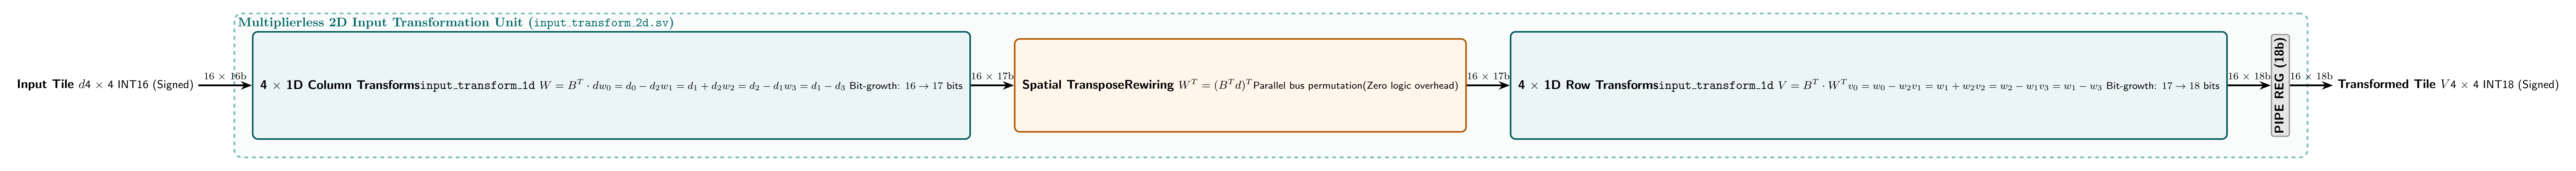
\includegraphics[width=0.95\textwidth]{input_transform_2d.png}
    \caption{Microarchitecture of the Multiplierless 2D Input Transform Unit (\texttt{input\_transform\_2d.sv}).}
    \label{fig:in_trans_diagram}
\end{figure}

The unit comprises:
\begin{itemize}
    \item \textbf{Four 1D Column Transform Blocks (\texttt{input\_transform\_1d}):} Operates concurrently on the 4 columns of tile $d$:
    \begin{align}
        w_0 &= d_0 - d_2 \\
        w_1 &= d_1 + d_2 \\
        w_2 &= d_2 - d_1 \\
        w_3 &= d_1 - d_3
    \end{align}
    All operations utilize purely signed 16-bit adders/subtractors with 1-bit sign extension to 17 bits.
    \item \textbf{Spatial Matrix Transposition:} Achieved entirely via hardwired bus routing (zero logic gate overhead and zero cycle delay).
    \item \textbf{Four 1D Row Transform Blocks:} Processes the transposed intermediate values to produce the 16-element matrix $V$ (18-bit signed), registered at the output.
\end{itemize}

\subsubsection{Parameterizable Multiplier Array (\texttt{multiplier\_array.sv})}
The multiplier engine executes the 16 element-wise multiplications $M_{i,j} = U_{i,j} \times V_{i,j}$ ($i,j \in \{0, 1, 2, 3\}$). The architecture supports architectural parameterization via the \texttt{PARALLEL\_DSPS} parameter:
\begin{itemize}
    \item \textbf{Full Parallelism ($N = 16$ DSPs):} Employs 16 physical multipliers operating in parallel, completing the entire $4 \times 4$ tile in a single clock cycle.
    \item \textbf{Half Parallelism ($N = 8$ DSPs):} Utilizes 8 time-multiplexed multipliers over 2 clock cycles, reducing DSP consumption by $50\%$ on resource-constrained FPGAs.
    \item \textbf{Quarter Parallelism ($N = 4$ DSPs):} Computes across 4 clock cycles using 4 DSP slices to minimize silicon area.
\end{itemize}
Outputs are registered as signed 34-bit values before entering the channel accumulator.

\subsubsection{Channel Accumulator Unit (\texttt{channel\_accumulator.sv})}
This module instantiates sixteen 36-bit accumulation registers governed by two control flags:
\begin{itemize}
    \item When \texttt{first\_channel = 1'b1}: The accumulators overwrite current values directly with new products $M$ (clearing previous tile history).
    \item When \texttt{first\_channel = 1'b0}: The unit adds incoming products to the running accumulator:
    \begin{equation}
        M_{\text{accum}}[i][j] \Leftarrow M_{\text{accum}}[i][j] + M[i][j]
    \end{equation}
    \item When \texttt{last\_channel = 1'b1}: The accumulator asserts \texttt{valid\_out = 1'b1}, signaling the output transform unit to process the completed accumulation matrix.
\end{itemize}

\subsubsection{2D Output Transform Unit (\texttt{output\_transform\_2d.sv})}
The 2D output transform converts the accumulated $4 \times 4$ matrix $M_{\text{accum}}$ (36-bit) into the final $2 \times 2$ output patch $Y$ (16-bit). Figure~\ref{fig:out_trans_diagram} depicts the microarchitecture.

\begin{figure}[htbp]
    \centering
    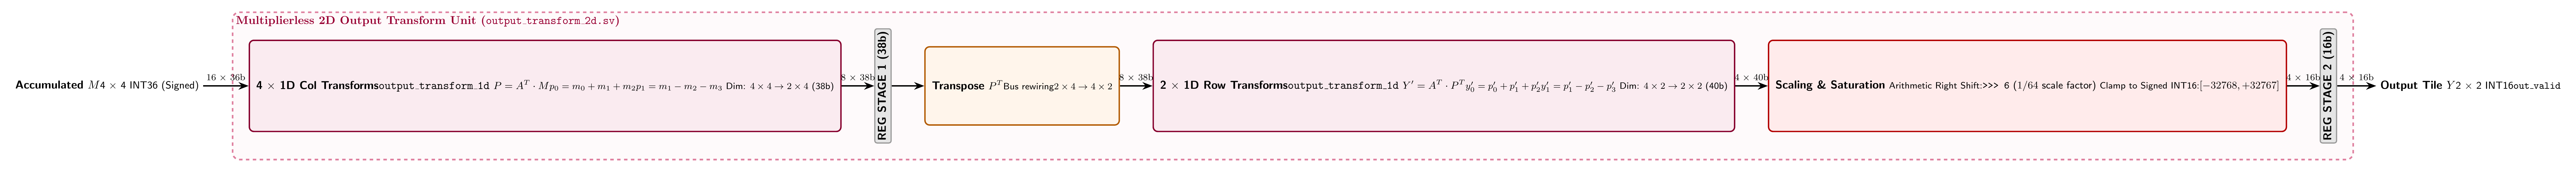
\includegraphics[width=0.98\textwidth]{output_transform_2d.png}
    \caption{Microarchitecture of the 2D Output Transform Unit with Requantization and Saturation (\texttt{output\_transform\_2d.sv}).}
    \label{fig:out_trans_diagram}
\end{figure}

The unit is structured into two pipelined stages to break lengthy combinational paths:
\begin{itemize}
    \item \textbf{Stage 1 - Column Transformation:} 4 instances of \texttt{output\_transform\_1d} compute $P = A^T \cdot M$:
    \begin{align}
        p_0 &= m_0 + m_1 + m_2 \\
        p_1 &= m_1 - m_2 - m_3
    \end{align}
    Transforming $4 \times 4 \to 2 \times 4$ matrices with bit expansion from 36 to 38 bits, stored in Stage 1 pipeline registers.
    \item \textbf{Stage 2 - Row Transformation:} Hardwired transpose yields $P^T$ ($4 \times 2$), followed by 2 instances of \texttt{output\_transform\_1d} computing $Y' = A^T \cdot P^T$ ($2 \times 2$, 40 bits).
    \item \textbf{Stage 3 - Requantization and Symmetrical Saturation:} The 40-bit results are arithmetically right-shifted by 6 bits (\texttt{>>> 6}) and clamped to signed INT16 boundaries ($[-32768, 32767]$), asserting \texttt{out\_valid} upon completion.
\end{itemize}

\subsubsection{FSM Controller (\texttt{winograd\_controller.sv})}
The control unit coordinates multi-channel accumulation sequencing and handshake synchronization through a 4-state finite state machine illustrated in Figure~\ref{fig:fsm_diagram}.

\begin{figure}[htbp]
    \centering
    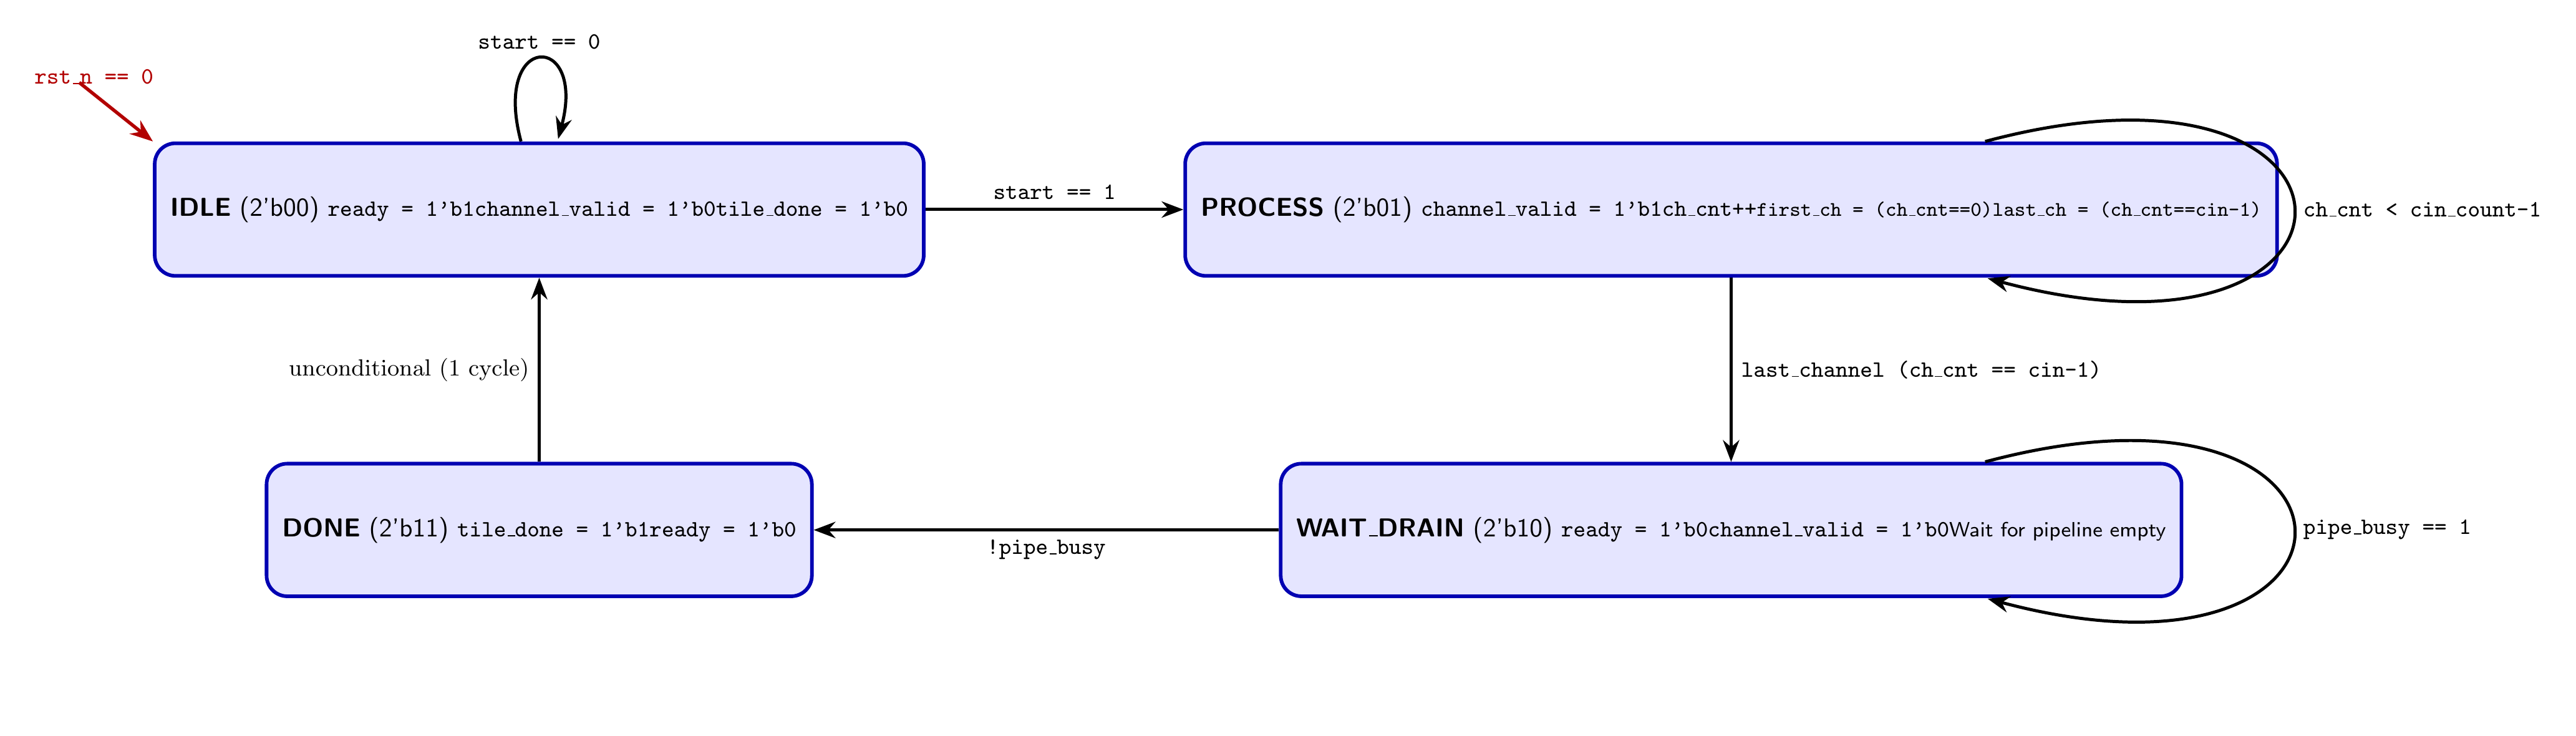
\includegraphics[width=0.85\textwidth]{winograd_fsm.png}
    \caption{Finite State Machine (FSM) State Transition Diagram (\texttt{winograd\_controller.sv}).}
    \label{fig:fsm_diagram}
\end{figure}

The operational behavior of each state is defined as follows:
\begin{itemize}
    \item \textbf{IDLE (\texttt{2'b00}):} The core is quiescent, asserting \texttt{ready = 1'b1}. Upon detecting \texttt{start = 1'b1}, the channel counter \texttt{ch\_cnt} resets to 0, transitioning the FSM to \texttt{PROCESS}.
    \item \textbf{PROCESS (\texttt{2'b01}):} Asserts \texttt{channel\_valid = 1'b1} to stream channel data. Generates \texttt{first\_channel = (ch\_cnt == 0)} and \texttt{last\_channel = (ch\_cnt == cin\_count - 1)}. The counter increments until reaching the final channel, transitioning to \texttt{WAIT\_DRAIN}.
    \item \textbf{WAIT\_DRAIN (\texttt{2'b10}):} Deasserts \texttt{ready} and \texttt{channel\_valid}, waiting for internal pipeline stages to drain completely (\texttt{!pipe\_busy}).
    \item \textbf{DONE (\texttt{2'b11}):} Pulses \texttt{tile\_done = 1'b1} for one cycle to indicate tile completion, then returns unconditionally to \texttt{IDLE}.
\end{itemize}

% ==============================================================================
% SECTION 3: MÔ PHỎNG THIẾT KẾ / SIMULATION & VERIFICATION
% ==============================================================================
\section{Design Simulation and Verification}
\label{sec:simulation}

\subsection{Verification Methodology and Flow}
To ensure functional correctness, a hierarchical self-checking verification methodology was established, as outlined in Figure~\ref{fig:verif_flow}.

\begin{figure}[htbp]
    \centering
    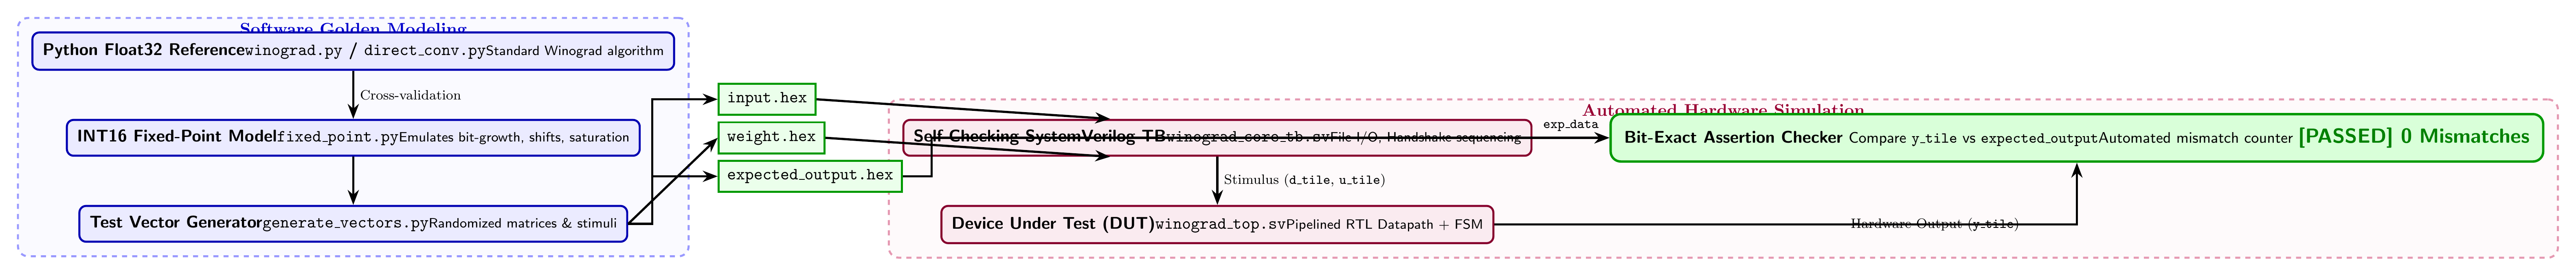
\includegraphics[width=\textwidth]{verification_flow.png}
    \caption{Hierarchical Simulation and Verification Methodology Flow.}
    \label{fig:verif_flow}
\end{figure}

The verification strategy encompasses three rigorous steps:
\begin{enumerate}
    \item \textbf{Software Reference Modeling:}
    \begin{itemize}
        \item \texttt{python/winograd.py}: Formulates standard Winograd Float32 convolution using transformation matrices $B^T, G, A^T$ and cross-validates against \texttt{direct\_conv.py}.
        \item \texttt{python/fixed\_point.py}: Accurately emulates hardware fixed-point behavior, including bit-growth expansion, arithmetic shift scaling (\texttt{>>> 6}), and symmetrical clamping saturation.
    \end{itemize}
    \item \textbf{Automated Test Vector Generation:} The \texttt{python/generate\_vectors.py} script produces randomized feature map activations and kernel weights, evaluates them through the fixed-point reference model, and exports three synchronized hex stimulus files:
    \begin{itemize}
        \item \texttt{tb/input.hex}: Raw $4 \times 4$ signed 16-bit input activations.
        \item \texttt{tb/weight.hex}: Pre-transformed $4 \times 4$ signed 16-bit weights ($U = G g G^T$).
        \item \texttt{tb/expected\_output.hex}: Golden $2 \times 2$ output activations.
    \end{itemize}
    \item \textbf{Self-Checking SystemVerilog Testbench:} The top-level testbench \texttt{tb/winograd\_core\_tb.sv} reads the hex files via \texttt{\$readmemh}, drives the DUT through valid/ready handshakes, monitors \texttt{y\_tile} outputs, and performs cycle-by-cycle automated assertion comparison. Any bit discrepancy increments an internal mismatch counter.
\end{enumerate}

\subsection{Unit-Level Simulation Verification}
Before executing full core regressions, each sub-module was verified in isolation:
\begin{itemize}
    \item \textbf{Input Transform Unit (\texttt{input\_transform\_tb.sv}):} Tested against corner-case stimuli (all maximum $+32767$, all minimum $-32768$, and alternating sign patterns). Confirmed correct 18-bit expansion without overflow, achieving \textbf{0 mismatches}.
    \item \textbf{Output Transform Unit (\texttt{output\_transform\_tb.sv}):} Validated 1D/2D add-trees, shift scaling, and saturation bounds. Whenever intermediate values exceeded $\pm 32767$, values clamped accurately to boundaries with zero sign-inversion errors.
\end{itemize}

\subsection{Top-Level Accelerator Core Simulation}

\subsubsection{Pipeline Timing and Waveform Analysis}
Figure~\ref{fig:pipeline_timing} illustrates the detailed pipeline timing diagram captured during multi-channel operation and continuous tile streaming.

\begin{figure}[htbp]
    \centering
    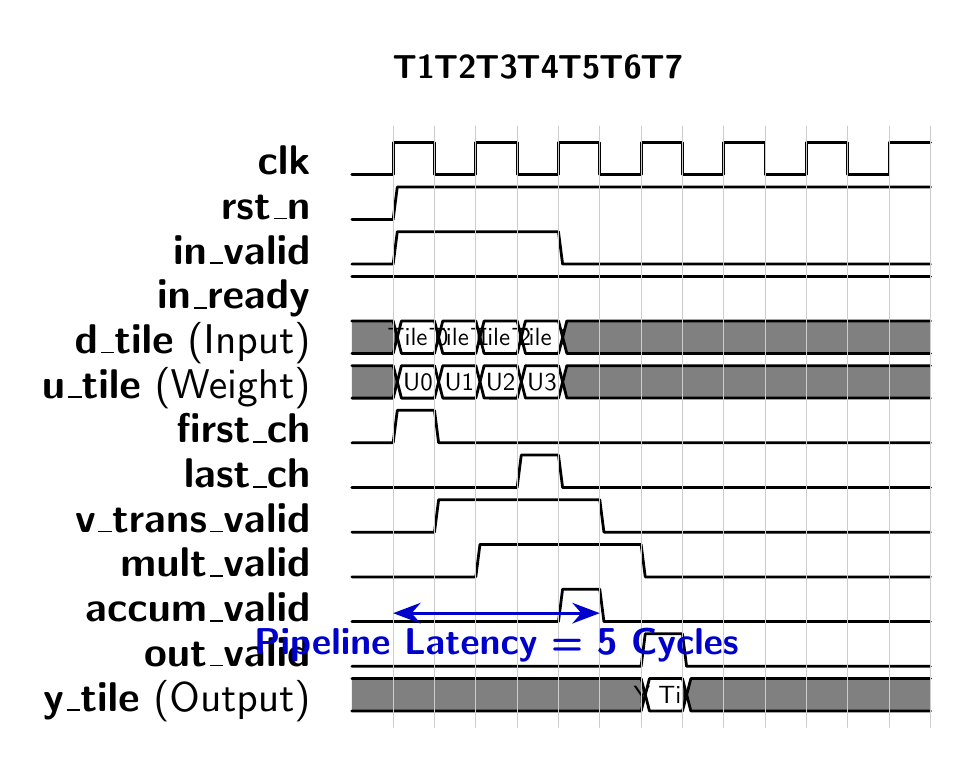
\includegraphics[width=\textwidth]{pipeline_timing.png}
    \caption{Pipeline Timing Diagram of the Winograd Accelerator Core.}
    \label{fig:pipeline_timing}
\end{figure}

Timing analysis reveals the following operational milestones:
\begin{itemize}
    \item \textbf{Cycle T1:} Reset deasserts (\texttt{rst\_n = 1'b1}), \texttt{in\_ready = 1'b1}. Valid inputs \texttt{d\_tile} and \texttt{u\_tile} are accepted with \texttt{first\_ch = 1'b1}.
    \item \textbf{Cycle T2 (1-cycle latency):} Input transform computes $V = B^T d B$, asserting \texttt{v\_trans\_valid = 1'b1}.
    \item \textbf{Cycle T3 (2-cycle latency):} Multiplier array completes 16 parallel multiplications $M = U \odot V$, asserting \texttt{mult\_valid = 1'b1}.
    \item \textbf{Cycle T5 (4-cycle latency):} Following 4 streamed input channels and assertion of \texttt{last\_ch}, the channel accumulator completes $M_{\text{accum}}$ and asserts \texttt{accum\_valid = 1'b1}.
    \item \textbf{Cycle T7 (6-cycle latency):} Output transform completes 2-stage row-column transformation, shift, and saturation, asserting \texttt{out\_valid = 1'b1} with valid $2 \times 2$ output tile \texttt{y\_tile}.
    \item \textbf{Initial Pipeline Latency:} Exactly \textbf{5 clock cycles} from the first valid tile presentation to corresponding output availability for a single-channel configuration.
    \item \textbf{Steady-State Throughput:} Once the pipeline is primed in single-channel mode, the accelerator outputs \textbf{1 complete $2 \times 2$ tile every clock cycle} (Throughput = 1 tile/cycle).
\end{itemize}

\subsubsection{Automated Regression Verification on ModelSim}
The verification testbench was compiled and simulated using ModelSim (Intel FPGA Edition 10.5b). Table~\ref{tab:sim_summary} provides the quantitative summary of the regression run across 50 test tiles (200 output pixels).

\begin{table}[htbp]
    \centering
    \caption{Summary of ModelSim Regression Verification Results.}
    \label{tab:sim_summary}
    \begin{tabular}{lc}
        \toprule
        \textbf{Verification Metric}                     & \textbf{Observed Result} \\
        \midrule
        Simulator Platform                               & ModelSim - Intel FPGA Edition 10.5b \\
        Hardware Description Language                    & SystemVerilog (IEEE 1800-2012) \\
        Total Tiles Evaluated                            & \textbf{50 tiles} \\
        Total Output Pixels Verified                     & \textbf{200 pixels} \\
        Total Mismatches Detected                        & \textbf{0} \\
        Initial Pipeline Latency                         & \textbf{5 clock cycles} \\
        Steady-State Throughput                          & \textbf{1 tile / clock cycle} \\
        Regression Status                                & \textbf{[PASSED] ZERO BIT MISMATCHES!} \\
        \bottomrule
    \end{tabular}
\end{table}

The simulation console transcript from ModelSim is shown below:
\begin{lstlisting}[caption={ModelSim Automated Regression Simulation Console Transcript.}]
# vsim -c winograd_core_tb -do "run -all; quit" 
# Loading work.winograd_core_tb
# Loading work.winograd_top
# Loading work.input_transform_2d
# Loading work.multiplier_array
# Loading work.channel_accumulator
# Loading work.output_transform_2d
# [TB] Loading hex test vectors...
# [TB] Test vectors loaded successfully.
# [TB INFO] Verified 10 / 50 tiles...
# [TB INFO] Verified 20 / 50 tiles...
# [TB INFO] Verified 30 / 50 tiles...
# [TB INFO] Verified 40 / 50 tiles...
# [TB INFO] Verified 50 / 50 tiles...
# 
# =======================================================
#           REGRESSION SIMULATION SUMMARY                
# =======================================================
#  Total Tiles Tested   : 50
#  Total Output Pixels  : 200
#  Total Mismatches     : 0
#  STATUS               : [PASSED] ZERO BIT MISMATCHES!  
# =======================================================
# ** Note: $finish    : tb/winograd_core_tb.sv
\end{lstlisting}

These simulation findings verify that the synthesizable SystemVerilog RTL core achieves bit-exact arithmetic accuracy, successfully satisfies all functional specifications, and is fully primed for subsequent physical synthesis and FPGA implementation.

% ==============================================================================
% REFERENCES
% ==============================================================================
\newpage
\begin{thebibliography}{99}
    \addcontentsline{toc}{section}{References}

    \bibitem{lavin2016}
    A.~Lavin and S.~Gray, ``Fast algorithms for convolutional neural networks,'' in \textit{Proceedings of the IEEE Conference on Computer Vision and Pattern Recognition (CVPR)}, pp.~4013--4021, 2016.

    \bibitem{winograd1980}
    S.~Winograd, \textit{Arithmetic Complexity of Computations}, vol.~33 of CBMS-NSF Regional Conference Series in Applied Mathematics, SIAM, Philadelphia, 1980.

    \bibitem{he2016resnet}
    K.~He, X.~Zhang, S.~Ren, and J.~Sun, ``Deep residual learning for image recognition,'' in \textit{Proceedings of the IEEE Conference on Computer Vision and Pattern Recognition (CVPR)}, pp.~770--778, 2016.

    \bibitem{lu2017fpga}
    L.~Lu, J.~Xie, R.~Huang, C.~Liu, and W.~Luk, ``An efficient hardware accelerator for sparse convolutional neural networks on FPGAs,'' in \textit{IEEE 25th Annual International Symposium on Field-Programmable Custom Computing Machines (FCCM)}, pp.~17--24, 2017.

    \bibitem{ieee1800}
    IEEE, \textit{1800-2017 - IEEE Standard for SystemVerilog--Unified Hardware Design, Specification, and Verification Language}, IEEE Standards Association, 2017.

\end{thebibliography}

% ==============================================================================
% APPENDIX
% ==============================================================================
\newpage
\begin{appendices}

    \section{Synthesizable SystemVerilog Module Snippets}
    \label{app:rtl_code}

    \begin{lstlisting}[language=Verilog, caption={Multiplierless 1D Input Transformation Stage in SystemVerilog (\texttt{input\_transform\_1d.sv}).}]
// =============================================================================
// Module: input_transform_1d
// Description: Multiplierless 1D Winograd input transform: V = B^T * d
// Formula:
//   v[0] = d[0] - d[2]
//   v[1] = d[1] + d[2]
//   v[2] = d[2] - d[1]
//   v[3] = d[1] - d[3]
// =============================================================================
module input_transform_1d #(
    parameter DATA_WIDTH = 16,
    parameter OUT_WIDTH  = 18
)(
    input  logic signed [DATA_WIDTH-1:0] d [0:3],
    output logic signed [OUT_WIDTH-1:0]  v [0:3]
);
    // Pure addition and subtraction trees (no DSP slices required)
    assign v[0] = $signed({{2{d[0][DATA_WIDTH-1]}}, d[0]}) - 
                  $signed({{2{d[2][DATA_WIDTH-1]}}, d[2]});
                  
    assign v[1] = $signed({{2{d[1][DATA_WIDTH-1]}}, d[1]}) + 
                  $signed({{2{d[2][DATA_WIDTH-1]}}, d[2]});
                  
    assign v[2] = $signed({{2{d[2][DATA_WIDTH-1]}}, d[2]}) - 
                  $signed({{2{d[1][DATA_WIDTH-1]}}, d[1]});
                  
    assign v[3] = $signed({{2{d[1][DATA_WIDTH-1]}}, d[1]}) - 
                  $signed({{2{d[3][DATA_WIDTH-1]}}, d[3]});
endmodule
\end{lstlisting}

    \section{Python Golden Model Reference Implementation}
    \label{app:python_code}

    \begin{lstlisting}[language=Python, caption={Python Winograd F(2x2, 3x3) Algorithmic Reference Implementation.}]
import numpy as np

# Fixed Winograd Transformation Matrices
BT = np.array([
    [ 1,  0, -1,  0],
    [ 0,  1,  1,  0],
    [ 0, -1,  1,  0],
    [ 0,  1,  0, -1]
], dtype=np.float32)

G = np.array([
    [ 1.0,  0.0, 0.0],
    [ 0.5,  0.5, 0.5],
    [ 0.5, -0.5, 0.5],
    [ 0.0,  0.0, 1.0]
], dtype=np.float32)

AT = np.array([
    [ 1,  1,  1,  0],
    [ 0,  1, -1, -1]
], dtype=np.float32)

def winograd_f2x2_3x3(d, g):
    """
    Computes Winograd F(2x2, 3x3) convolution on a 4x4 input tile d and 3x3 kernel g.
    Returns: 2x2 output tile Y.
    """
    # 1. Transform weights (pre-computed offline)
    U = np.matmul(np.matmul(G, g), G.T)
    # 2. Transform input tile (separable: B^T * d * B)
    V = np.matmul(np.matmul(BT, d), BT.T)
    # 3. Element-wise multiplication in transform domain (16 mults)
    M = U * V
    # 4. Output transformation (separable: A^T * M * A)
    Y = np.matmul(np.matmul(AT, M), AT.T)
    return Y
\end{lstlisting}

\end{appendices}

\end{document}
